%preámbulo
\documentclass[12pt,oneside,FLEQN]{report}
\usepackage{amssymb,amsthm,amsmath,enumerate,graphicx,tabularx}
\usepackage[utf8]{inputenc}
\usepackage[hidelinks]{hyperref}
\usepackage[spanish]{babel}
\usepackage[rflt]{floatflt}
\usepackage{multicol}
\usepackage{tcolorbox, empheq}
\tcbuselibrary{skins,breakable,listings,theorems}
\usepackage{tikz,tkz-tab}
\usetikzlibrary{matrix,arrows, positioning,shadows,shadings,backgrounds,calc, shapes, tikzmark}
\usepackage{subfigure}
\usepackage{caption}
\usepackage[a4paper]{geometry}
\geometry{top=1.5cm, bottom=1.5cm, left=3cm, right=3cm}
\usepackage{ragged2e}
\newcommand{\marcar}[3]{\tikz[overlay,remember picture,baseline=-2pt] \node[circle,#1,draw,text=black, inner sep=1pt] (#2) { #3};}
\parindent=0cm
\usepackage{listings}
\hypersetup{
colorlinks=true,
linkcolor=black,
filecolor=magenta,
urlcolor=cyan,
citecolor=greenwhats
}
\usepackage[dvipsnames,table]{xcolor}
%\usepackage{lscape}
\usepackage{enumitem}
\definecolor{greenwhats}{RGB}{37, 211, 102}
\definecolor{gris}{rgb}{0.33, 0.41, 0.47}
\usepackage{fancyhdr}
\usepackage{natbib}
\usepackage{colortbl}
\usepackage{array,booktabs}
%\usepackage{pdflscape}
\usepackage{longtable}
\definecolor{codeturquoise}{RGB}{72,202,228}
\definecolor{codeyellow}{RGB}{255,170,51}
\definecolor{codepurple}{RGB}{255, 203, 242}
\definecolor{codegreen}{RGB}{149,213,178}
\definecolor{backcolour}{RGB}{73,80,87}
\definecolor{white}{RGB}{255,255,255}
\lstdefinestyle{estilochidori}{
backgroundcolor=\color{backcolour},
commentstyle=\color{codeyellow},
keywordstyle=\color{codeturquoise},
numberstyle=\tiny\color{codegreen},
stringstyle=\color{codepurple},
basicstyle=\ttfamily\footnotesize\color{white},
breakatwhitespace=false,
breaklines=true,
captionpos=b,
keepspaces=true,
numbers=left,
numbersep=5pt,
showspaces=false,
showstringspaces=false,
showtabs=false,
tabsize=2
}
\lstset{style=estilochidori}
\begin{document}
{
\fontfamily{qag}\selectfont
\begin{titlepage}
        \topmargin=0cm
        \centering

        {\bfseries\LARGE Universidad Autónoma de Querétaro \par}
        \vspace{1cm}
        {\scshape\Large  Facultad de Ingenier\'ia  \par}
        \vspace{2cm}
        \centering
        \begin{figure}[!h]
        \centering
                
\includegraphics[height=5cm]{Logouaq.png}
        \end{figure}
        \vspace{3cm}
        {\itshape\large Tarea 9: Regresiones\par}
        \vspace{3cm}
        {\Huge Análisis numérico \par}
        \vspace{2cm}
        {\Large Autor: \par}
        {\large J.A. Salinas Sánchez \par}
        {\large Marzo 2022 \par}
\end{titlepage}
\tableofcontents
\chapter{Introducción}
En los capítulos anteriores, ya se vio el cómo; con una función, ecuación o expresión en general; se puede obtener datos de vital importancia en la resolución de diversos problemas; por más irresolvible que ésta pareciera. No obstante, si en lugar de tener la expresión matemática, se tiene los datos; para muchas ramas de la ciencia, economía, ingeniería y muchas otras áreas del conocimiento; obtener una expresión que permita generalizar el conocimiento y hacer predicciones, a partir de los datos; es construir y hacer nueva ciencia. Por ende, es muy importante.\\

Tal fue el caso de el muestreo del movimiento orbital de Ceres por el astrónomo italiano Piazzi, él tenía los datos de la posición del planeta enano en función del tiempo; pero no tenía la función del movimiento de Ceres en función del tiempo, por lo que era muy difícil hacer predicciones de su posición y modelar su órbita; el corazón de la astronomía. Fue entonces cuando el genio de Gauss se ideó una manera de obtener cualquier familia de funciones a través de un muestreo. Así nació la interpolación por mínimos cuadrados\\

El método se llama interpolación por mínimos cuadrados, ya que consiste en lo siguiente: obtener la distancia dos puntos de una función elegida arbitrariamente, evaluada en los datos del muestreo, y hacer la diferencia entre ésta y la distancia entre los puntos del muestreo sea mínima. En otras palabras, minimizar el error cuadrático de una función arbitraria evaluada en la muestra con la misma muestra. Para que quede claro: sacar los mínimos cuadrados para que una función cualquiera se parezca lo más posible a los datos; obtener una función a partir de los datos.

¿Y eso cómo se aprecia matemáticamente? Así:
\begin{align}
	a_{n}=\dfrac{n\sum_{k=1}^{n}(x_{k}y_{k})-\sum_{k=1}^{n}(x_{k})\sum_{k=1}^{n}(y_{k})}{n\sum_{k=1}^{n}x^{2}_{k}-(\sum_{k=1}^{n}x_{k})^{2}}\\
	b=\dfrac{\sum_{k=1}^{n}(y_{k})\sum_{k=1}^{n}(x^{2}_{k})-\sum_{k=1}^{n}(x_{k})\sum_{k=1}^{n}(x_{k}y_{k})}{n\sum_{k=1}^{n}x^{2}_{k}-(\sum_{k=1}^{n}x_{k})^{2}}
\end{align}
Donde a son los coeficientes de la variable independiente de la función, y b, el término independiente. En el caso de que la función sea diferente de la línea recta, simplemente a cada $x_{k}$ se le irá aplicando la función siguiente hasta evaluar $f(x_{k})$, es decir, se evaluará en la función arbitraria elegida, o se irá construyendo hasta llegar a la función polinomial elegida ($x^{n}$).
\chapter{Método}
	\section{Código}
		El código consiste en un script que recibe el tamaño de la muestra, pide la introducción de cada dato para x e y, y el número n+1 de regresiones polinomiales que se desea evaluar. Luego, evalúa todas las regresiones polinomiales que se le indicó, la logarítmica y la exponencial; las grafica y regresa la gráfica y la función. Esto lo hice así, pues este código está pensado para ser parte de un programa mayor, en el cual se le introduzca una muestra y un factor de correlación $r$ deseado, y que el programa evalúe todas las posibles regresiones hasta hallar la correcta y devolverla. NOTA: sigue en trabajo.
		\lsinputlisting{regpoli.py}
	\section{Ejercicios}
		\subsection{17.5}
			\begin{figure}[!h]
				\centering
				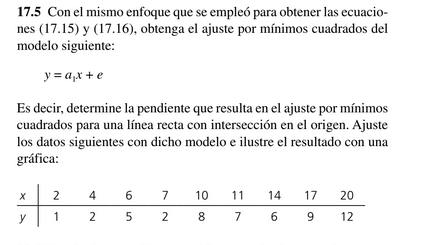
\includegraphics[scale=0.5]{175e.png}
				\caption{}
			\end{figure}
			\begin{figure}[!h]
				\centering
				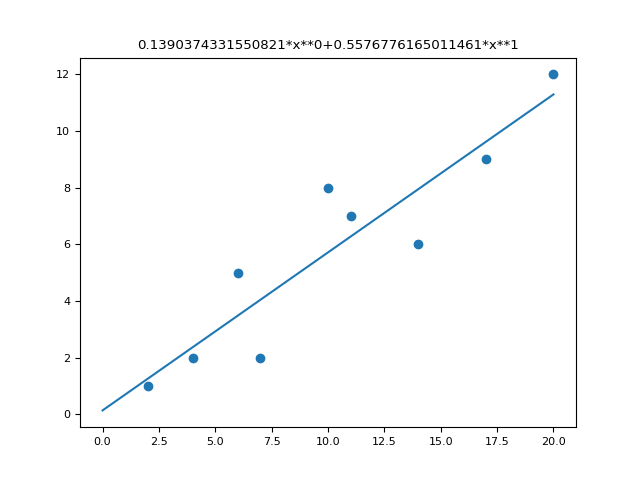
\includegraphics[scale=0.3]{175.png}
				\caption{Gráfica con la línea de tendencia y los puntos graficados}
			\end{figure}
		\subsection{17.9}
			\begin{figure}[!h]
				\centering
				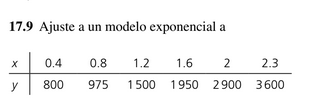
\includegraphics[scale=0.5]{179e.png}
				\caption{}
			\end{figure}
			\begin{figure}[!h]
				\centering
				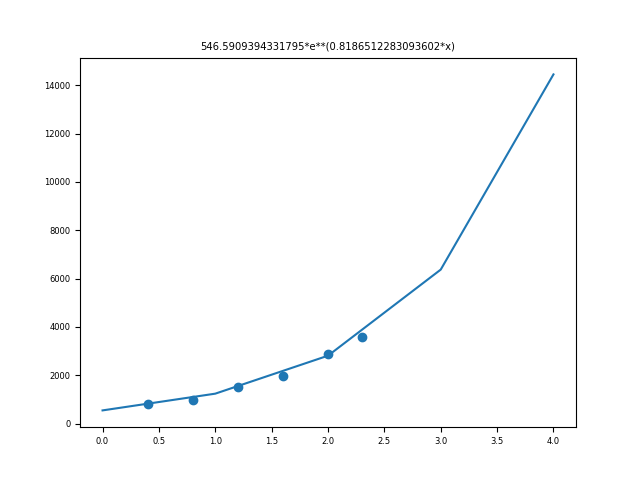
\includegraphics[scale=0.3]{179.png}
				\caption{Gráfica con la línea de tendencia y los puntos graficados}
			\end{figure}
		\subsection{17.17}
			\begin{figure}[!h]
				\centering
				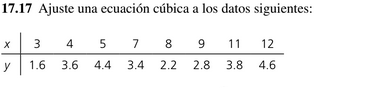
\includegraphics[scale=0.5]{1717e.png}
				\caption{}
			\end{figure}
			\begin{figure}[!h]
				\centering
				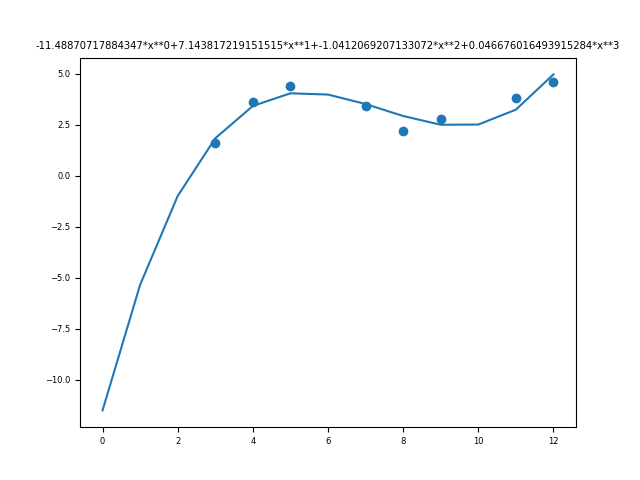
\includegraphics[scale=0.3]{1717.png}
				\caption{Gráfica con la línea de tendencia y los puntos de la muestra}
			\end{figure}
		\subsection{17.28}
			\begin{figure}[!h]
			\begin{figure}[!h]
				\centering
				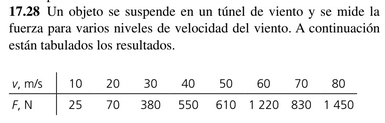
\includegraphics[scale=0.5]{1728e.png}
				\caption{}
			\end{figure}
				\centering
				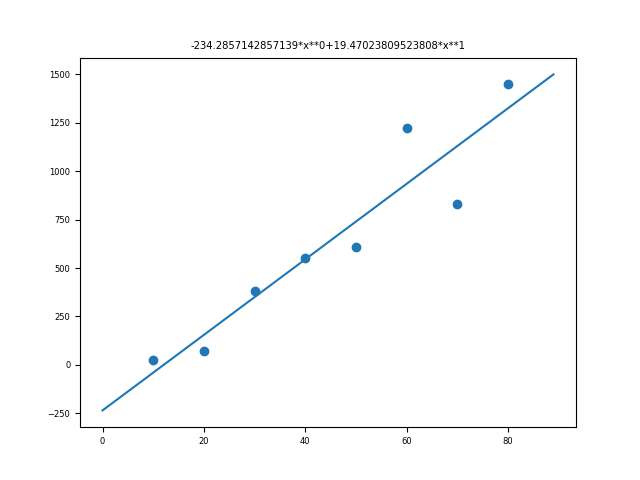
\includegraphics[scale=0.3]{17281.png}
				\caption{Gráfica de la interpolación lineal y los puntos de la muestra}
			\end{figure}
			\begin{figure}[!h]
				\centering
				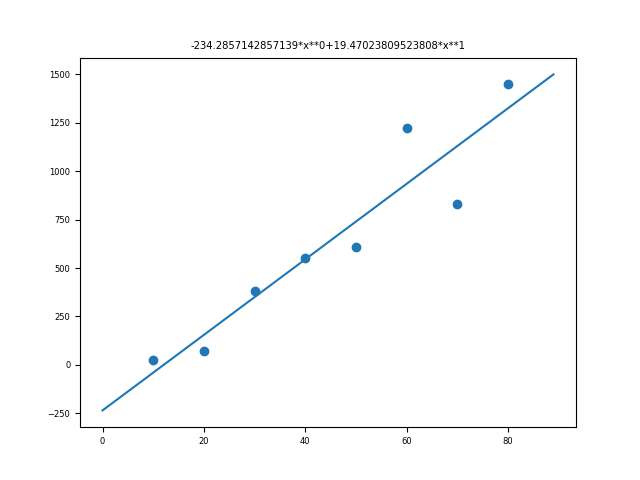
\includegraphics[scale=0.3]{17281.png}
				\caption{Gráfica de la interpolación exponencial y los puntos de la muestra}
			\end{figure}

\chapter{Conclusión}
Como se vio, para cualquier área del conocimiento, es necesario obtener modelos matemáticos, pues es lo que vuelve al conocimiento empírico en teórico, y el teórico en empírico. Es lo que permite volver al conocimiento empírico en algo concreto, preciso y predecible; y al teórico, en predicciones, mediciones y cantidades significativas al momento de resolver problemas. Porque, si bien se puede deducir nueva teoría de los modelos ya existentes, éstos pudieron venir de datos experimentales o de modelos teóricos que, a su vez, requirieron verificación experimental. Con esto, quiero concluir utilizando dos citas de grandes genios de la física y de toda la historia de la humanidad:
{\it No importa qué tan bella sea tu teoría, ni cuán listo seas. Si no concuerda con el experimento, está mal.}-R.P. Feynman- porque {\it Las matemáticas son el idioma con el que Dios ha escrito el Universo}-G. Galilei- y, añadiendo una mía, {\it... entonces, si tu experimento realmente representa la naturaleza del cosmos; tal como dijo Galileo, tiene que tener una representación matemática simple y elegante; y si tu representación matemática simple  elegante realmente representa al Universo; tiene que tener evidencia experimental}. 

}
\end{document}
